\section{Architecture} % (fold)
\label{sec:architecture}
CC is a software suite that provides the building blocks for creating power aware clusters. It consists of various software pieces that maintain the set of nodes in the cluster and automatically turn them off when they are idle in order to save power. It is completely written in python and the complete set of files is about 700 lines of code (not including existing software like \emph{Ganglia} and \emph{wakeonlan}).

\subsection{Ganglia} % (fold)
\label{sub:ganglia}
\begin{figure}[ht]
\centering
\begin{center}
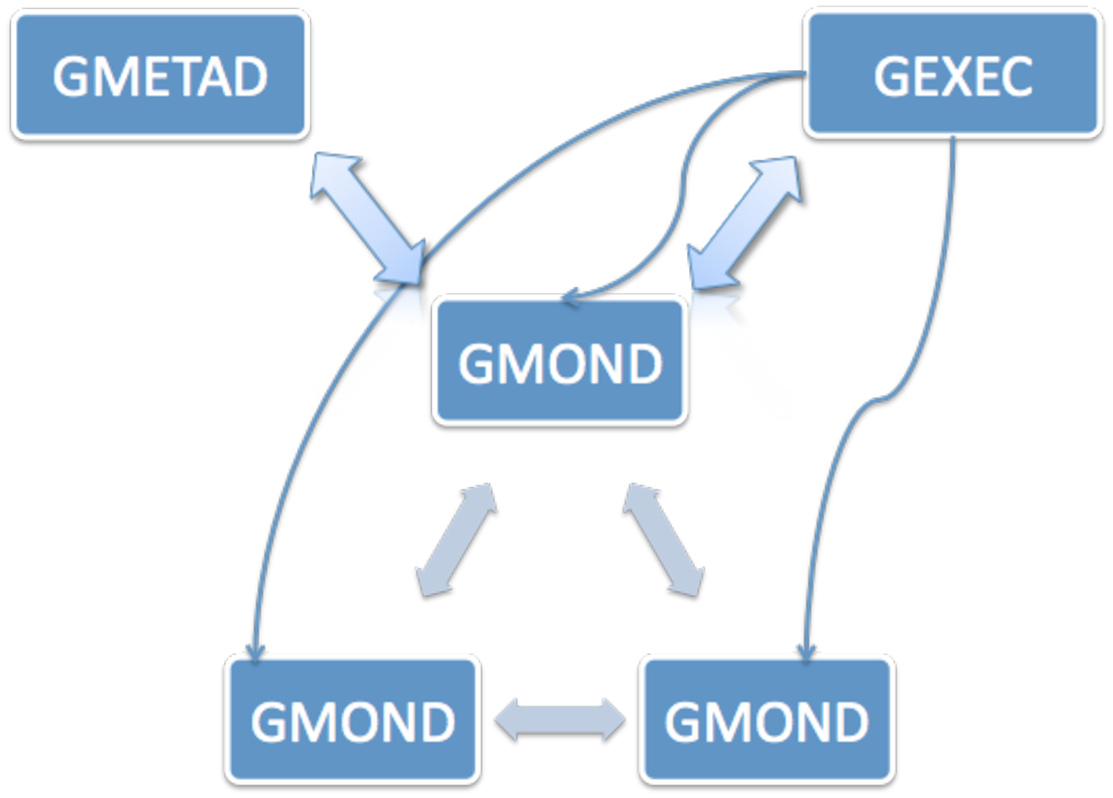
\includegraphics[width=3.0in]{graphs/ganglia-arch.pdf}
\vspace{-0.1in}
\caption{{\normalsize Architecture of the Ganglia cluster monitoring suite}\label{fig:ganglia-arch}}
\vspace{-0.1in}
\end{center}
\end{figure}
Ganglia is a widely used cluster monitoring software. We use ganglia in order to do the collection of resource statistics on individual nodes in the system. A Google web search for "ganglia report" pages produces more than a thousand hits. From this, it can be inferred that Ganglia is a widely used monitoring software installed on clusters and grids around the world. Ganglia uses a completely distributed no-master architecture. It consists of the following modules:
\begin{description}
    \item[gmond] is a daemon that resides on each node in the cluster and routinely publishes the resource characteristics of the system on a UDP multicast channel. All nodes in the cluster also subscribe to the same multicast channel, hence each of the nodes in the cluster maintains a recent snapshot of the state of the cluster.
    \item[gmetad] is a data collection and visualization daemon. It subscribes to the multicast channel and usually stores information for longer periods of time. It is also responsible for converting the data into a human readable format and updating a web application for humans to view.
    \item[rrd] (Round Robin Database) is a widely used database format used for storing time series data. Both gmond and gmetad store the data locally in rrd files. The advantage of this data structure is that the oldest data is automatically discarded or easily aggregated.
    \item[authd] is an authentication daemon which runs on all nodes of the cluster that are capable of running cluster jobs. It is responsible for authenticating jobs issued by a valid scheduler.
    \item[gexec] is a simple, no frills cluster job scheduler that hooks into the gmond servers to get a list of active nodes in the cluster. It then connects to {\bf gexecd} on those nodes in order to execute a command on all nodes in parallel.
\end{description}

% subsection ganglia (end)

\subsection{Clean Clusters (CC)} % (fold)
\label{sub:cleanclusters_cc_}
\begin{figure}[ht]
\centering
\begin{center}
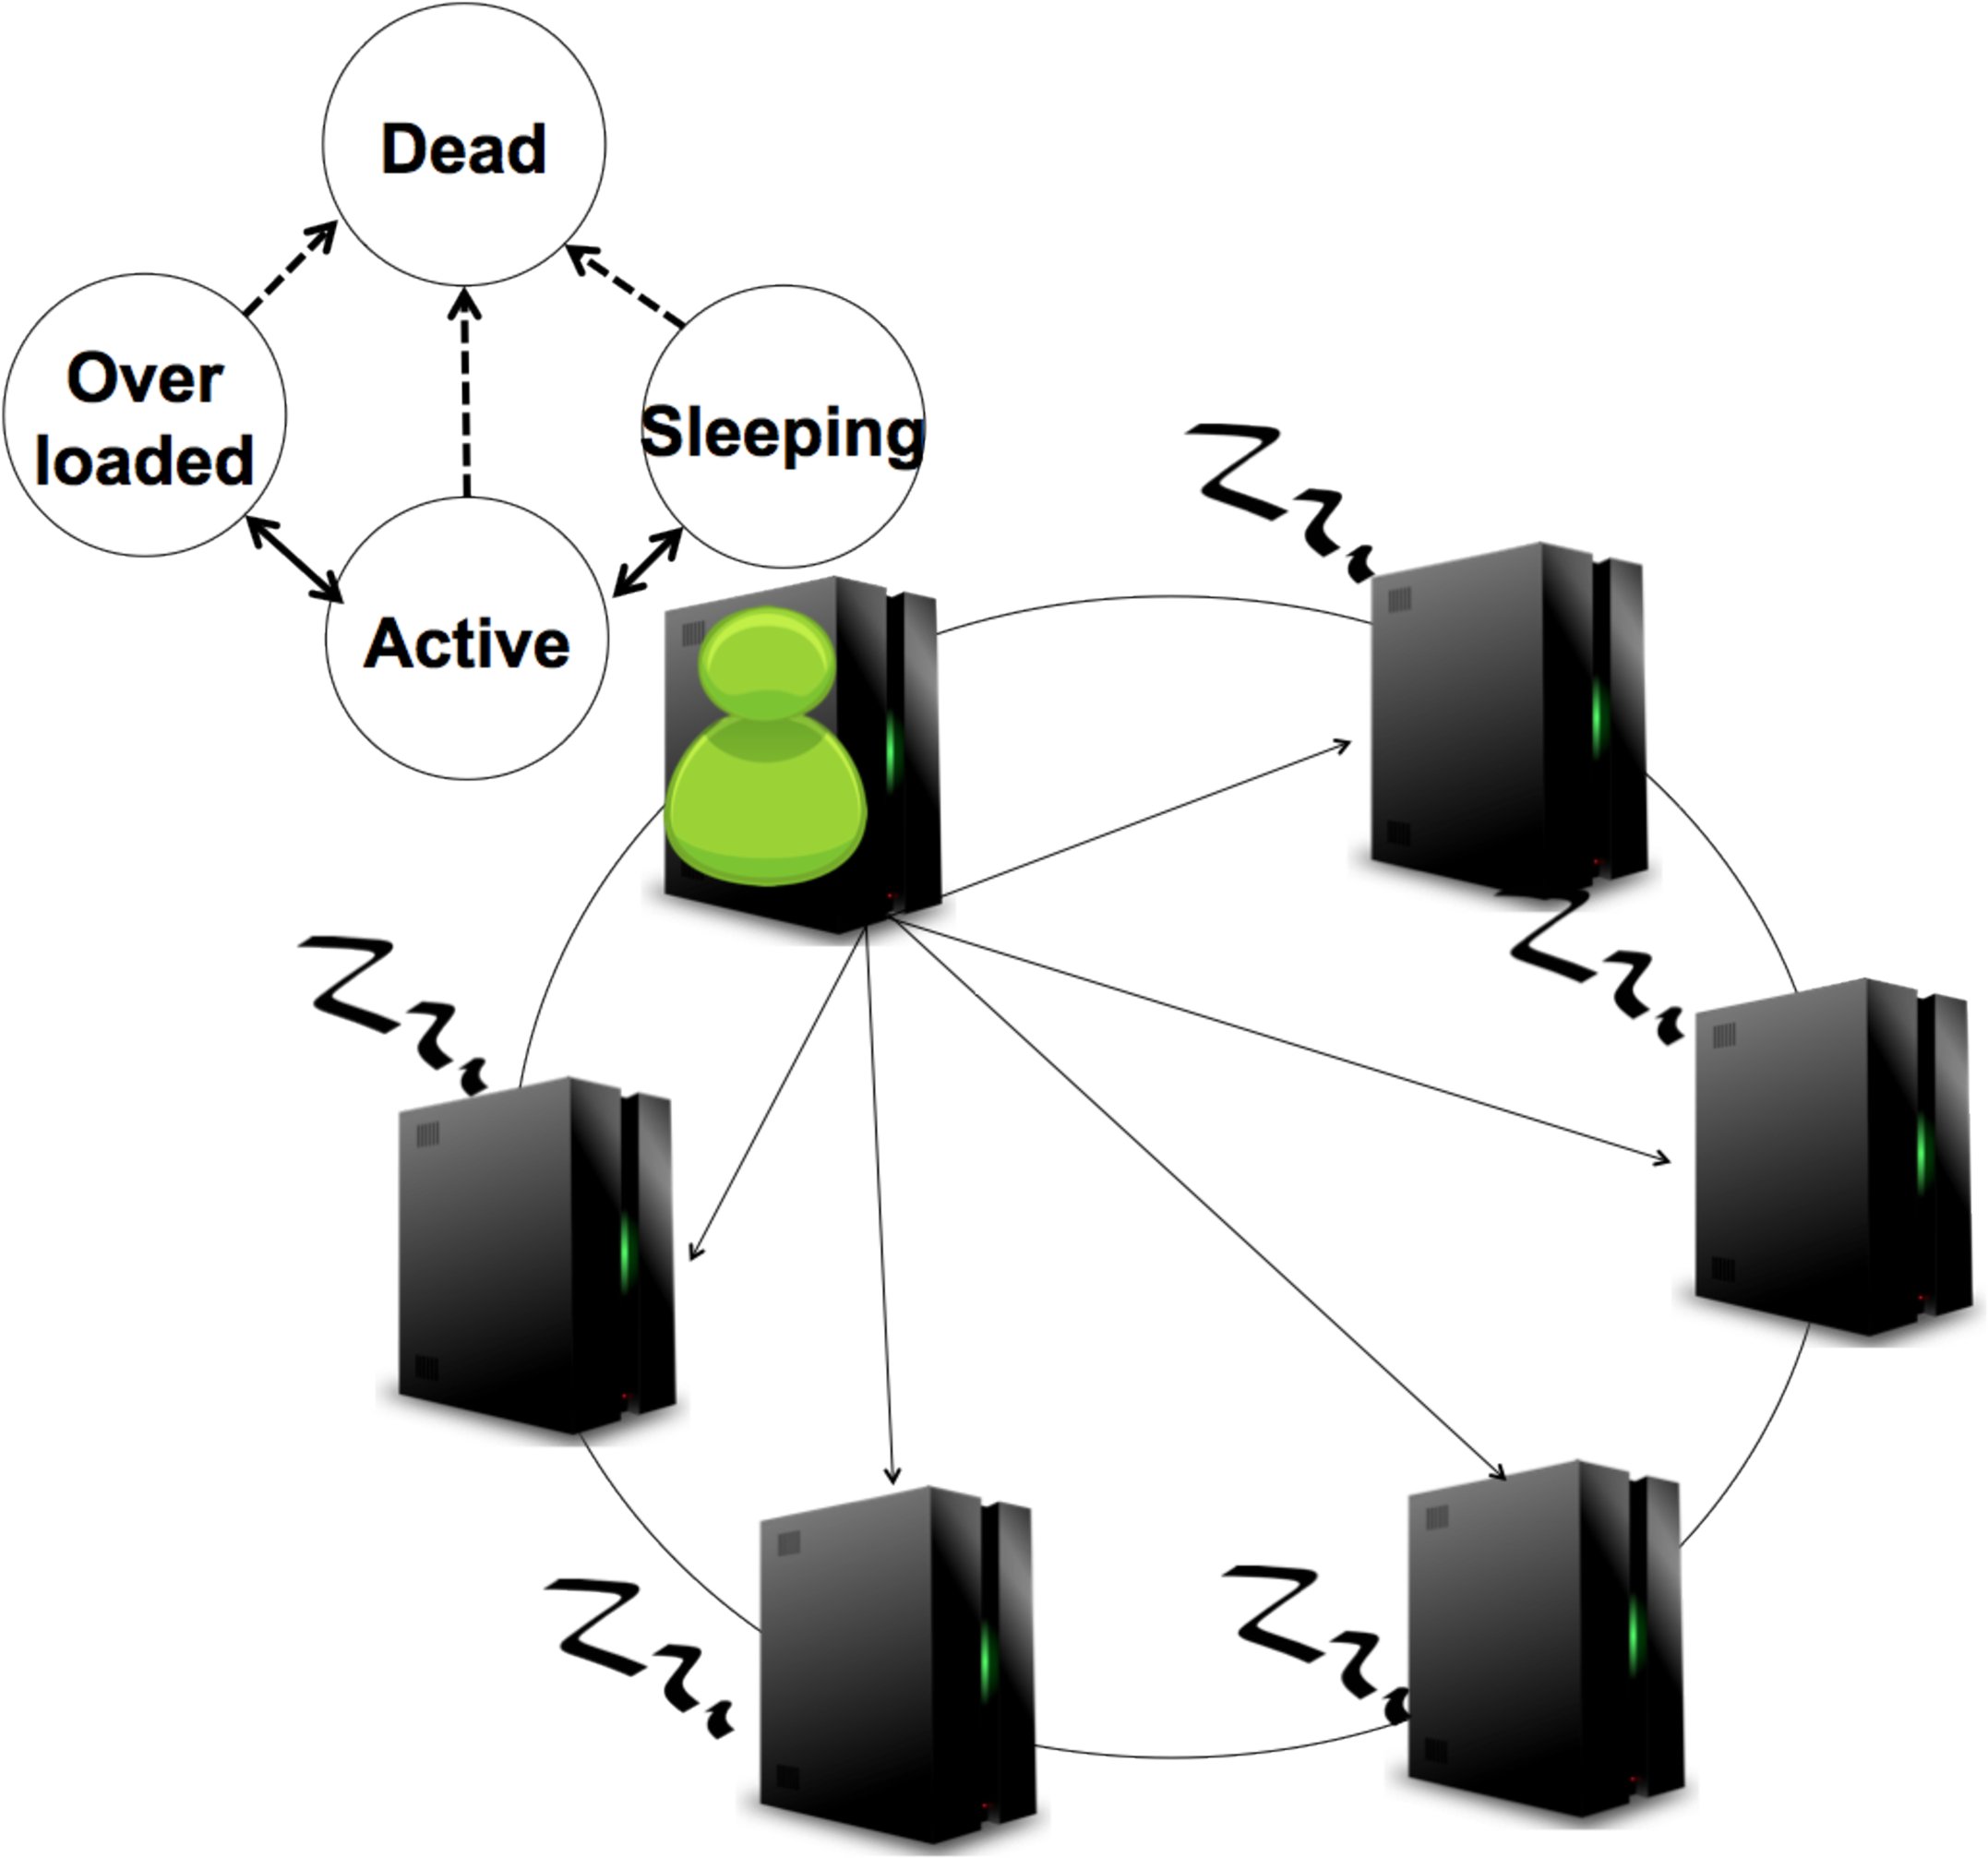
\includegraphics[width=2.5in]{graphs/CCd-arch.pdf}
\vspace{-0.1in}
\caption{{\normalsize Architecture of the Clean Cluster suite}\label{fig:cc-arch}}
\vspace{-0.1in}
\end{center}
\end{figure}

\begin{description}
    \item[Sleep Service] is implemented as a plugin to gmetad. The sleep service runs in one or more nodes in the cluster, listening to all ganglia messages. It maintains the set of nodes in the cluster and their state (sleeping/dead/active/overloaded). It routinely broadcasts it's IP address on the network for schedulers to be able to query the service. 
    \item[CCd] is a daemon which runs on each of the nodes in the cluster. If it is started with the `--sleep' option, then it will put the nodes to sleep automatically when there are no jobs running. Before putting the node to sleep, it publishes an intent to sleep as part of ganglia's messages. It then waits for any of the sleep services to acknowledge receipt of the intent before going to sleep. The program should either be setuid to {\em root} or should be run with sudo permissions in order for the sleep action to be successful.
\end{description}

\subsubsection{CCexec} % (fold)
\label{ssub:ccexec}
CCexec is a simple cluster scheduler akin to `gexec', however it makes use of the power saving nature of the CC suite. CCexec takes as input the number of instances of a command to run and the command itself. It then contacts the sleep service for information about the state of the cluster and then builds 4 queues based on the state of the nodes:
\begin{description}
    \item[active] - The active queue contains nodes which are currently awake and perhaps running jobs, but are still underutilized. 
    \item[sleeping] - The sleeping queue is the list of nodes which are currently suspended to ram. They had earlier published a sleep intent and are no longer reachable.
    \item[dead] - This queue contains a list of nodes that are currently un-reachable and had not published an intent to sleep earlier. It should be noted that even in the case of network partitions, each partition will continue to act as separate clusters where nodes from the other cluster are put in the dead queue. Once the partition is rectified, the cluster converges quickly to its original configuration. If a sleeping node does not respond to repeated wake up messages, it is assumed to be dead. 
    \item[overloaded] - The overloaded queue is the set of nodes that are awake and running jobs. These nodes are sufficiently utilized and are the last candidates for subsequent jobs unless any of the current jobs finish.
\end{description}

When a new job is submitted to the system using CCexec, each of the queues are populated and node allocation is first done from the active queue, then from the sleep queue (since there is an associated overhead of waking up the machine). 

% subsubsection ccexec (end)

% subsection subsection_name (end)

% subsection cleanclusters_cc_ (end)


% section architecture (end)